% Copyright 2010, Piotr Jakubowski

\chapter{Introduction}
  \section{Problem Description}
  Along with the huge popularization of the Internet there appeared enormous market for all sorts of web applications. Every month big companies, as well as small startups, try to get as much of this market by bringing in new features and shocking the crowd with innovative functionalities. Surprisingly, the market seems to be far from saturation as brilliant ideas except for fulfilling known demand create new needs as well.

  New tools started to emerge in order to meet the needs of Internet population. Dynamic languages started to supersede old and known. Python and Ruby became the new Java and C. The speed of development surpassed the speed of execution as technical limitations and price of servers are not the issue any more. Moreover, web development frameworks made it possible to code the application on the new level of abstraction - we can instantaneously start to implement our business logic, without the need to think about how we should persist our entities into database and how we should handle requests and respond to them. Java developers got Spring and Hibernate, but the noteworthy Ruby on Rails took web development to the whole new level. The threshold of making the ideas happen has been successfully shrunken.
  
  As mentioned before, today's software development has been focused on the effectiveness and speed of development. A lot of work has been done to create developer-oriented tools that try to make developing business ideas effortless.
  
  Of course, there is plenty of room for improvements. One of them is the idea of automating process of creating the administration panel for the application. Very often administration part of the application is mundane collection of CRUD\footnote{Create Read Update Delete} actions. It is the "must do" part. 
  
   User-oriented features is the target thing of development. This is what makes money and keeps us all employed. It seems like possibility to be able to automatically generate panel for administering our resources would make development of web application even more dynamic. It would bring plenty of benefits, such as:
  
  \begin{itemize}
	  \item Whole team can focus on what really matters, which is creating functionality that would be an added-value for users of the application
	  \item Adding new features and resources to the application would require less effort - as soon as the user-oriented functionality is ready the administration part is automatically generated.
	  \item Business people connected with the project can instantly browse new resources in the application.
	\end{itemize}
  
  Thereby, the aim of this thesis is to create and demonstrate the process of creation of plugin that would enable automatic generation of administration part of the application. The plugin would be developed for Ruby on Rails framework mentioned before.
  
  \section{Existing Solutions}
  Thanks to its rapidly growing popularity, Ruby and Ruby on Rails got very broad community. Not only does it result in a huge number of places you can ask for help, but also in all kind of libraries that would make the life of web developer easier. And as it seems I am not alone stating the issue described above. There are already several implementations attacking the problem of admin interface. Some of them are more successful than others, there are different kinds of approaches and different outcomes. 
  
  In order to see what market has to offer I looked through available solutions and chose 4 most popular ones in order to see what kind of functionalities they provide and what flaws they suffer from. 
  
    \subsection[Active Scaffold] {Active Scaffold\footnote{http://activescaffold.com/}}
      According to Ruby Toolbox\footnote{http://ruby-toolbox.com/categories/rails\_admin\_interfaces.html} it is the most popular plugin for admin interface generation. Unfortunately, it seems like the days of glory for this gem are long gone. The plugin does not support Rails in version 3, which despite being released very recently already became a standard for new applications. 
      
      Technicalities aside, it seems to be quite functional. The almost out-of-the-box look is presented on figures \ref{activescaffold1} and \ref{activescaffold2}
      \begin{figure}[hbt!]
    		\begin{center}
    			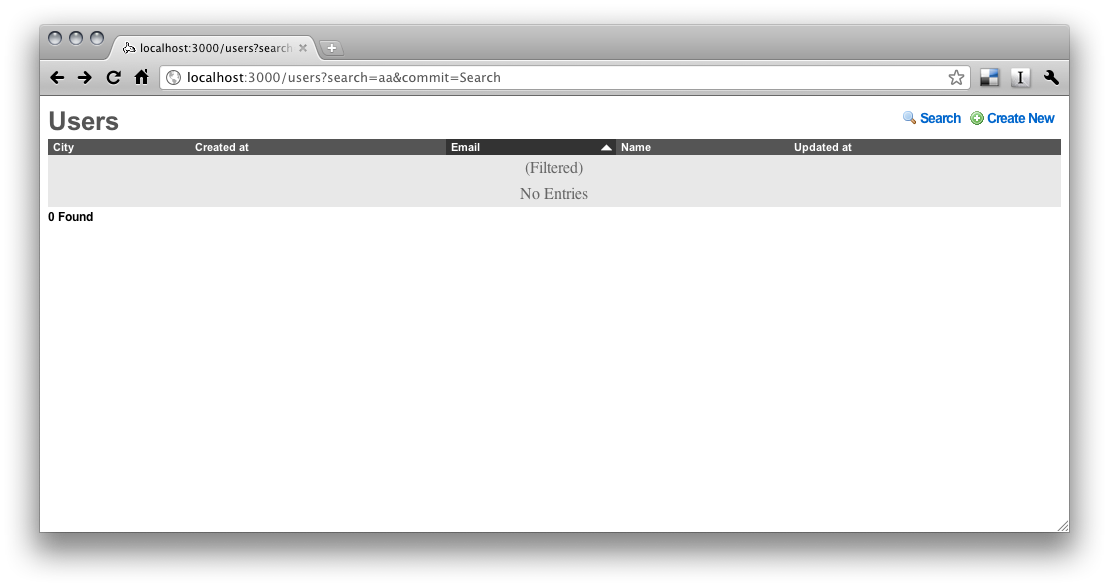
\includegraphics[width=\linewidth]{images/chapter01/activescaffold1.png}
    			\caption{Active Scaffold}
    			\label{activescaffold1}
    		\end{center}
    	\end{figure}
    	
    	\begin{figure}[hbt!]
    		\begin{center}
    			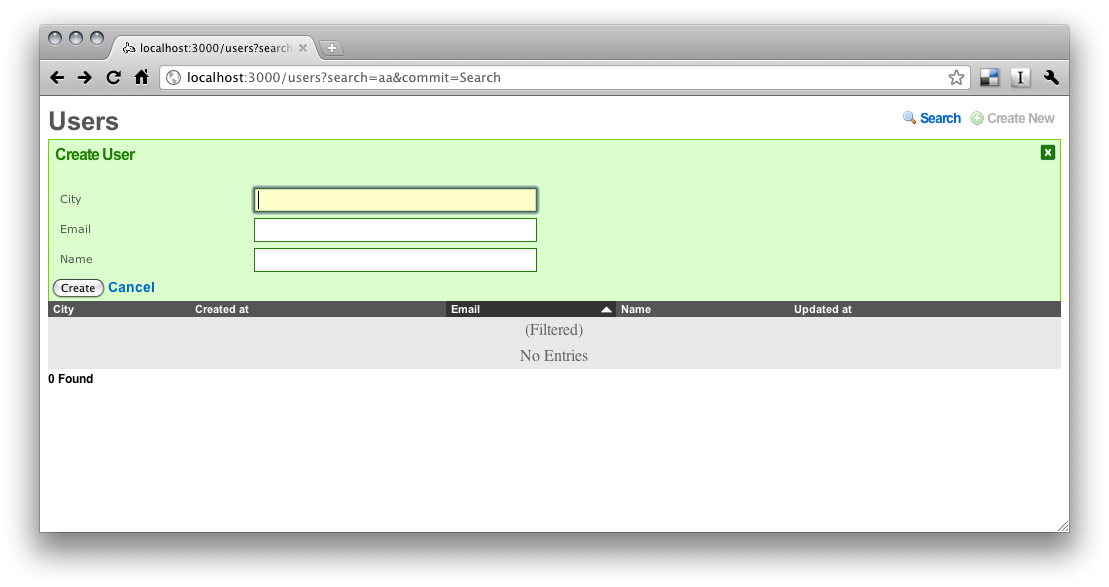
\includegraphics[width=\linewidth]{images/chapter01/activescaffold2.png}
    			\caption{Automatically generated form in Active Scaffold}
    			\label{activescaffold2}
    		\end{center}
    	\end{figure}
      
    Active Scaffold ships with comprehensive API for customizing its behavior. User can change which columns are visible in which view or how the system behaves during particular actions. Moreover, it uses \acrodef{AJAX}{Asynchronous JavaScript and XML} \ac{AJAX} for interaction with user which gives nice and responsive user interface.
    
    Unfortunately, it has big disadvantage. It is not entirely automatic. It requires developer to take following action to set it up:
    
    \begin{itemize}
      \item Add command to the layout of the application that will include styles and javascript for Active Scaffold.
      \item For every resource he wants to administer, he needs to create controller and add code that will set it up.
      \item Set up url for Active Scaffold actions for given controller by adding code to routes file.
    \end{itemize}

    This results in following inconveniences:
    
    \begin{itemize}
      \item Active Scaffold mixes with our application code.
      \item Every time we create some model we need to take care to set up Active Scaffold for it.
    \end{itemize}
    
    It seems like Active Scaffold instead of being "stand-alone" solution for administration is a set of commands, that speeds up set up of administration interface. It gives flexibility, but is not as hassle-free as could be and as developers would like it to be.
    
    \subsection[Typus] {Typus\footnote{http://core.typuscms.com/}}
    Typus is reported to be the second most popular Rails admin interface generator. As opposed to Active Scaffold, its development team is still active. Thanks to that, it has been adapted to Rails 3 already.
    
    Installation and set up is quick and effortless. We just need to install Typus and run one command. That way we get to the /admin path in our application. Its user interface is presented on figures \ref{typus1} and \ref{typus2}.
    
    \begin{figure}[hbt!]
  		\begin{center}
  			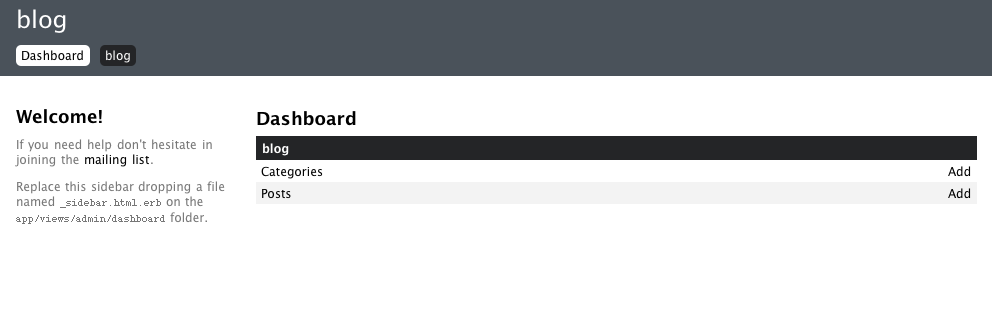
\includegraphics[width=\linewidth]{images/chapter01/typus1.png}
  			\caption{Typus main page}
  			\label{typus1}
  		\end{center}
  	\end{figure}
  	
  	\begin{figure}[hbt!]
  		\begin{center}
  			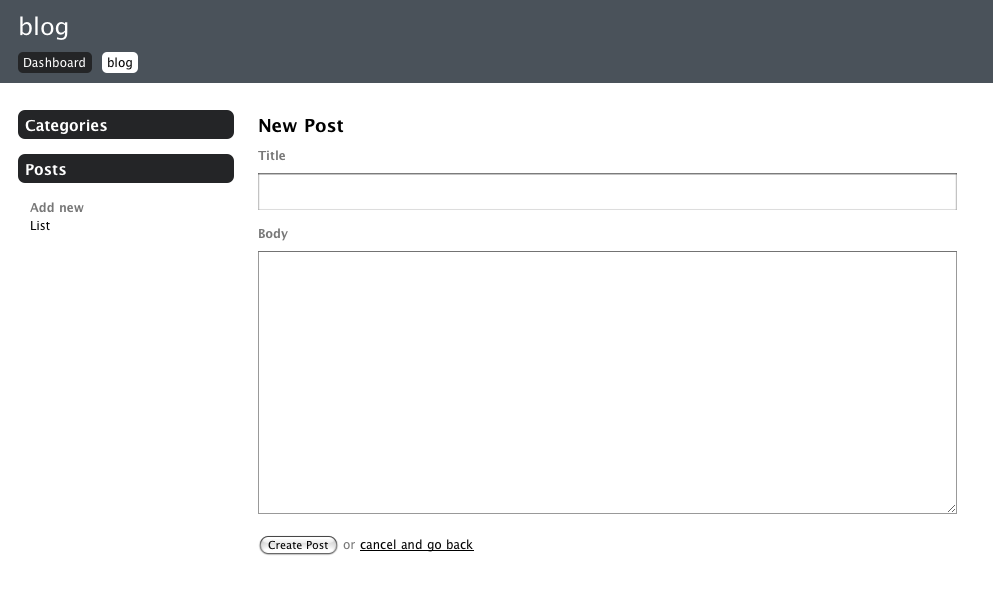
\includegraphics[width=\linewidth]{images/chapter01/typus2.png}
  			\caption{Automatically generated form in Typus}
  			\label{typus2}
  		\end{center}
  	\end{figure}
  
    Documentation provides thorough description of possibilities of Typus' customization. We can decide which columns will be visible, how admins can search our models and so on. Most of the configuration is done by specifying appropriate YAML files. In addition, Typus is supposed to handle file uploads in your application, which is very convenient. However, it will happen only if your application is using particular plugin for files upload called Paperclip.
    
    But again, similiar as it was in Active Scaffold, Typus does not work entirely "on-the-fly". The generator we have to run in order to set Typus up, except for copying needed HTML, javascript and image files, creates controllers that serve particular Models of our application. As said before, this means that we can get full control on how given controller behaves - we can override Typus implementation with our own - but such approach is not as dynamic in terms of adapting to upcoming resources in the application. Of course, now it is just the sake of running simple command that would take care of everything once we introduce some new Model into application, but surely it is not something we just install and can forget about.
    
    \subsection{admin\_data}
    Admin\_data is next one on the list. Again, the project seems to be still maintained and has been upgraded to Rails 3 already. Installation is very much alike to the one of Typus. But, after installation we do not need to run any generators or create any kind of files. We instantly get access to /admin\_data path and figure \ref{admindata1} presents what more or less we would see after trying it out.
     
    \begin{figure}[hbt!]
  		\begin{center}
  			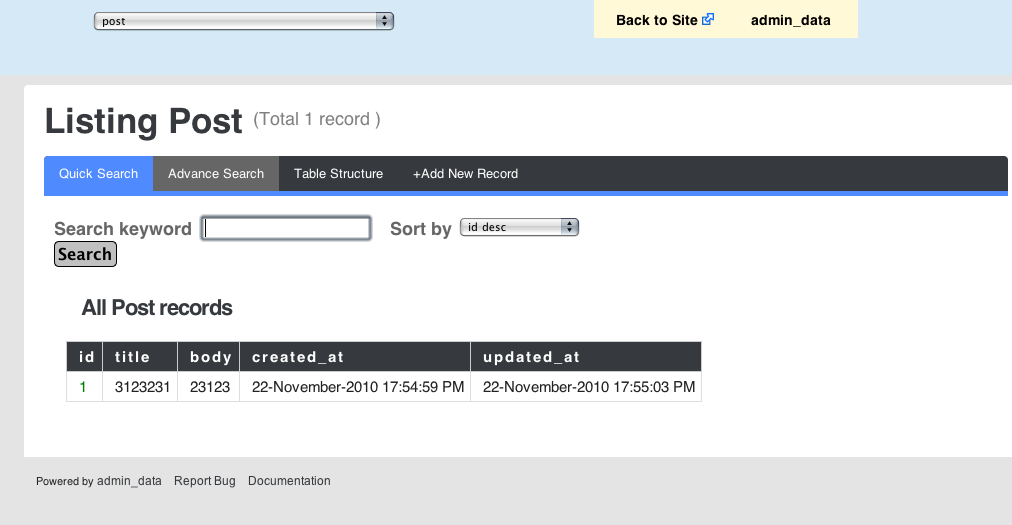
\includegraphics[width=\linewidth]{images/chapter01/admindata1.png}
  			\caption{Admin data}
  			\label{admindata1}
  		\end{center}
  	\end{figure}
  
  Of course, it provides us with some level of customizability, though it is not as wide as in two other projects. But, admin\_data has the level of dynamism I have been looking for. It creates the list of models on the fly, so while developing our application we will constantly have the most current version of our models lists, no question asked. Moreover, we can also see table's structure for given model, which may come in handy at times.
  
  On the other hand, you can clearly see that admin\_data has been created with programmers in mind. The user interface can be very hard to comprehend for people that do not know what is SQL or do not care how developers organized tables in the database. Therefore, it could be very hard to convince our business people that it is something they can use.
  
  \subsection{rails\_admin}
  Although rails\_admin is not present on the ruby-toolbox list it has been very popular lately. It has been developed during Ruby Summer of Code\footnote{http://rubysoc.org/}. It has been developed strictly for Rails 3 so it uses all the best features and the best practices from the newest version of the framework.
  
  Installation is very quick, although we need to go through few steps. Moreover, it depends on devise\footnote{https://github.com/plataformatec/devise} gem, which takes care of users authentication, as rails\_admin's default option is to make people to log in to the administration panel.
  
  What we get after installation is very nice and user-friendly panel(figure \ref{railsadmin1}). In addition, it tracks changes in records, what gives us functionality of seeing whole history of activities on records as well as people that made them. Additionally, we have that data presented in form of nice graph that gives us an idea of what was happening in the system throughout the month or year.
  
  
  \begin{figure}[hbt!]
		\begin{center}
			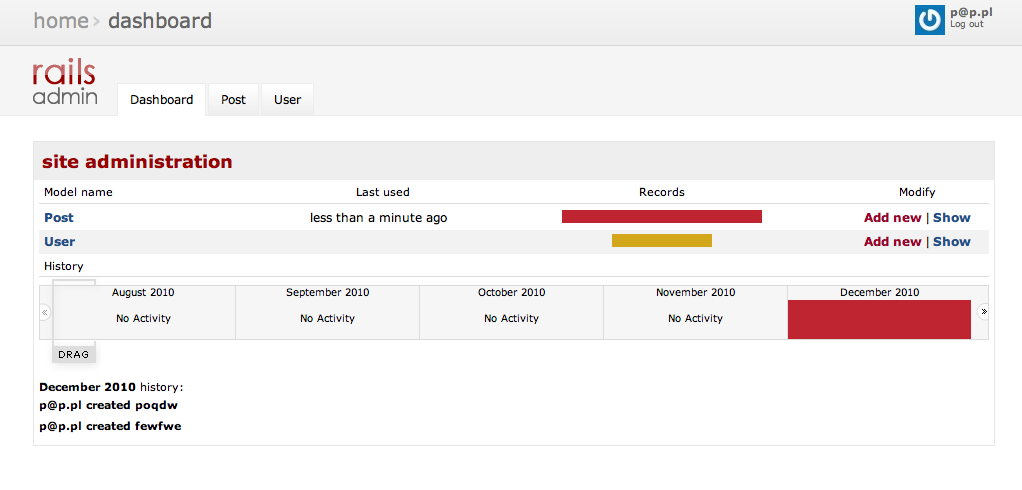
\includegraphics[width=\linewidth]{images/chapter01/railsadmin1.png}
			\caption{rails\_admin dashboard}
			\label{railsadmin1}
		\end{center}
	\end{figure}
	
	\begin{figure}[hbt!]
		\begin{center}
			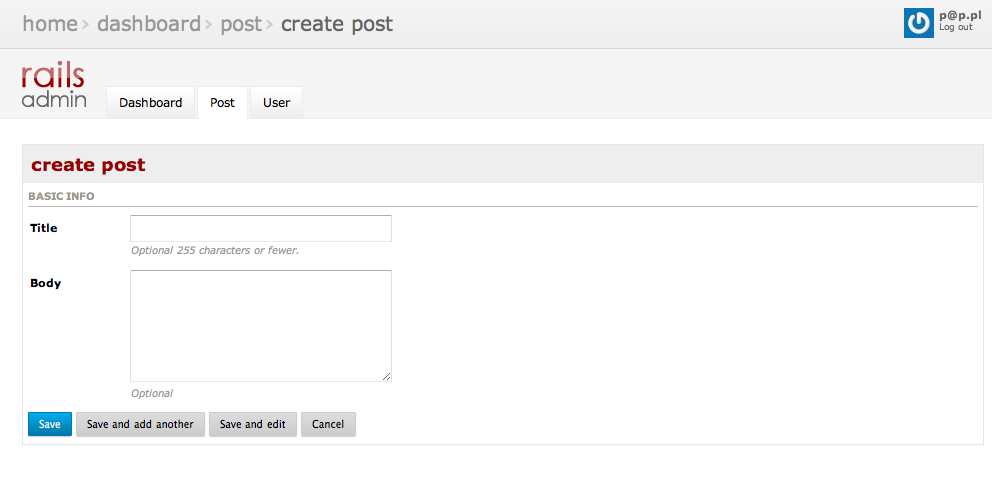
\includegraphics[width=\linewidth]{images/chapter01/railsadmin2.png}
			\caption{Form generated in rails\_admin }
			\label{railsadmin2}
		\end{center}
	\end{figure}

  Rails\_admin seems to have real potential and although I have not seen it in use in production yet, soon it maybe become real power of Rails applications. Definitely, ideas used in that project are very interesting and may be very useful.
  
  \section{Solution Proposal}
    \subsection{Solution Proposal}
    TBD
  
    \subsection{Projected Challenges}
    TBD